\chapter{Feature Extraction}
Feature extraction is the process of collecting relevant information from each data sample (object windows), which will be unique based on the class of the data sample. Features define each object uniquely in a satellite image. Features can help to differentiate between the objects and non-objects. We extract features from the potential object windows to predict if the window contains the object or not. 
\par In this survey, we have only focused on deep learning based feature extraction techniques, e.g, CNN.


\section{Convolutional Neural Networks (CNN)}
Convolutional neural networks is a type of feed-forward neural network which is specifically designed for features extraction from images. CNN has two types of layers, using which it can perform the forward and backward propagation. 
\par Forward propagation is performed by doing convolution operation on the pixels of the image with different number of filters and apply a non-linear activation function (e.g, ReLu) on the result along with a bias term. Here, the filters act as weight for the images. The result is given in figure \ref{fig6}.

\begin{figure}[!htbp]
\centerline{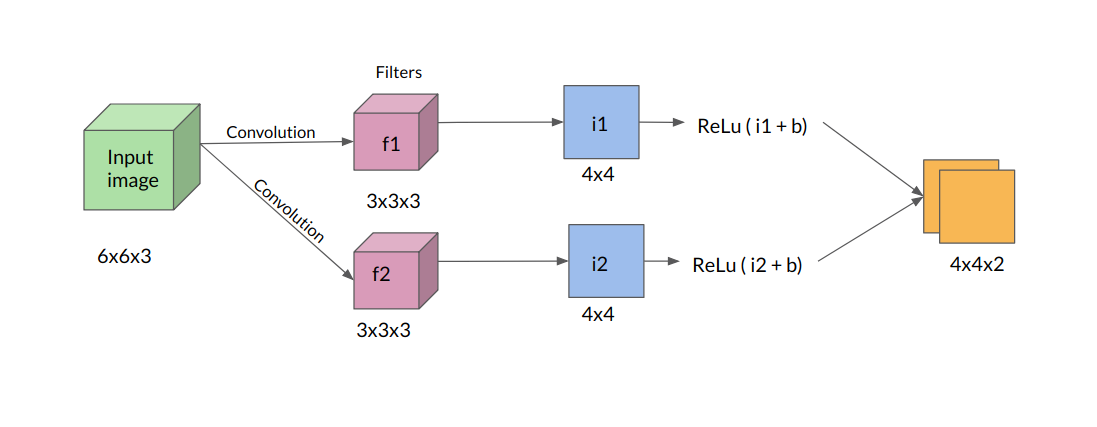
\includegraphics[height=80mm,width=160mm]{img/fig6.png}}
\caption{Result of one layer of convolution operation}
\label{fig6}
\end{figure}

\par The result from each filter is clubbed together and forwarded to the pooling layer. Pooling layers will reduce the size of the feature representation and speed up the computation. There are several kinds of pooling layers, e.g, max-pooling, average pooling etc. In max-pooling we apply filter on the input which will perform max operation. It is similar to previous step, only difference is that, instead of convolution we perform max operation. Example of max pooling is given in figure \ref{fig7}. 

\begin{figure}[!htbp]
\centerline{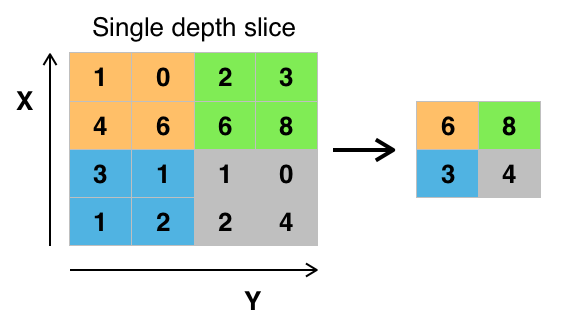
\includegraphics[height=50mm,width=85mm]{img/fig7.png}}
\caption{Result of max-pooling operation. Source: https://en.wikipedia.org}
\label{fig7}
\end{figure}

In average pooling we perform the averaging operation on the input. The general architecture of the CNN is given in figure \ref{fig8}.

\begin{figure}[!htbp]
\centerline{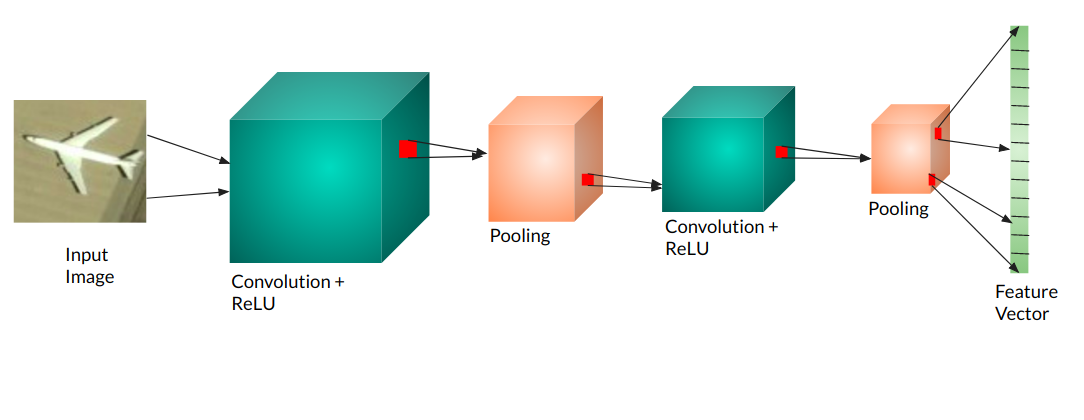
\includegraphics[height=60mm,width=150mm]{img/fig8.png}}
\caption{General architecture of a CNN}
\label{fig8}
\end{figure}

At the last layer we will get a volume of specific size as output. Let the size of this volume is $m\times n\times p$. Then this volume will be flattened to a vector of feature of dimension $[m\times n\times p, 1]$. This feature vector will be forwarded to the classification stage.

\par Wu et.al. \cite{b5} has used CNN architecture for feature extraction. They have created a model with 4 layers. The architecture is C-S-C-S, where C is convolutional layer and S is pooling layer. $32\times 32$ sized images has been given as input to the architecture. The filter size at convolutional layer is $5\times 5$ and size of pooling filter is $2\times 2$.


\section{CNN with Histogram Oriented Gradients (HOG)}
Zhang et.al \cite{b6} has used this combined method for feature extraction. They have done oil-tank detection in satellite images. It has been observed that the surrounding of an oil-tank consists of shadows, trees, pipelines and other oil-tanks. So, the authors has used CNN to extract this surrounding feature and HOG to extract the local feature of the oil-tank. Local feature means the feature of the oil-tank only. As there could be many oil-tank like circular objects present in satellite images, thus the authors has used both these features to correctly detect and localize the oil-tanks. 
\par We have already discussed about CNN in the above section, thus in this section we will describe the HOG feature calculation process.
\subsection{Histogram Oriented Gradients (HOG)}
HOG can accurately represent the information about the shape of an object present in an image. The main idea behind HOG is that the distribution of gradient orientation has the capacity to accurately detect and characterize the appearance of the objects. 
\par Feature descriptor of an image fetches out the important information and eliminates the excess informations. It converts the image into a flat vector of features. HOG \cite{b7} feature descriptor takes $64\times 128$ images as input. First the input is pre-processed by performing gamma correction. 
\par Then, the horizontal and vertical gradients are calculated using filters. The filtering is done by using horizontal and vertical kernel shown in figure \ref{fig9}.

\begin{figure}[!htbp]
\centerline{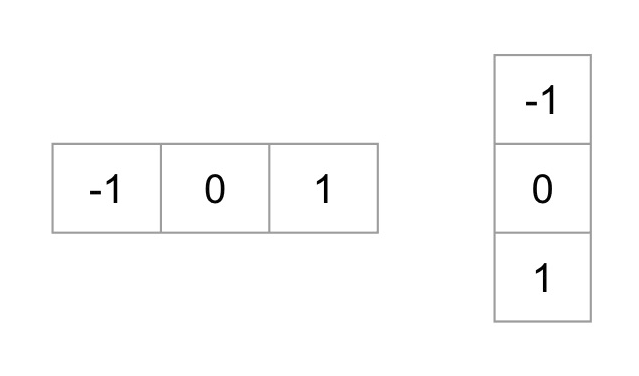
\includegraphics[height=60mm,width=120mm]{img/fig9.png}}
\caption{Horizontal and vertical kernels. Source: https://www.learnopencv.com}
\label{fig9}
\end{figure}

By using horizontal and vertical gradients we can calculate the modulus and direction of the gradient using the formula:
$$g=\sqrt{(g_x)^2+(g_y)^2},\ \theta=tan^{-1}(\frac{g_y}{g_x})$$ where $g_x$ is the horizontal gradient and $g_y$ is the vertical gradient. $g$ is the gradient modulus and $\theta$ is the gradient direction.

\par Now we divide the images into cells of size $8\times 8\times 3$ pixels, where $3$ is the number of channels, i.e, R,G, B. We calculate the gradient for each of these cells using the process described above. After gradient calculation, the cell is converted to size $8\times 8\times 2=128$ values. This is depicted in figure \ref{fig10}. 

\begin{figure}[!htbp]
\centerline{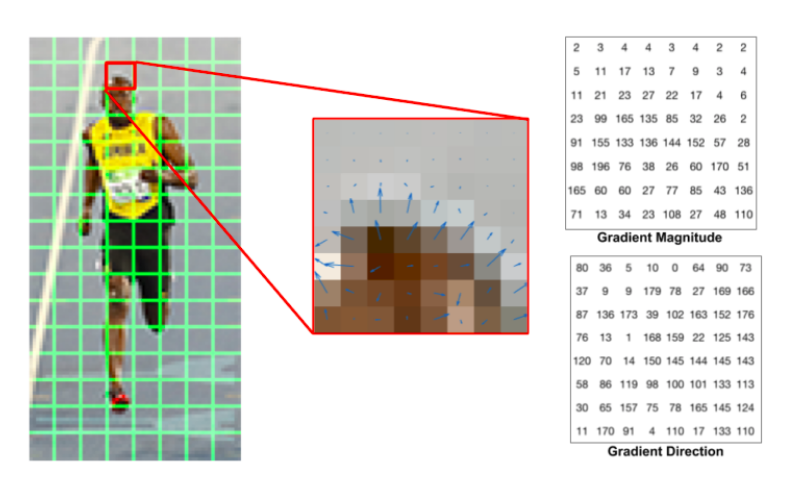
\includegraphics[height=90mm,width=150mm]{img/fig10.png}}
\caption{Conversion of cells into gradients. Source: https://www.learnopencv.com}
\label{fig10}
\end{figure}

These 128 values are represented using a 9-bin histogram. The 9-bin histogram is an array of 9-numbers corresponding to angles 0, 20, 40, 60,..., 160. Now, based on the gradient direction matrix we put the corresponding values from gradient modulus matrix to a particular position of the 9-bin histogram array. This mapping is depicted in figure \ref{fig11}.

\begin{figure}[!htbp]
\centerline{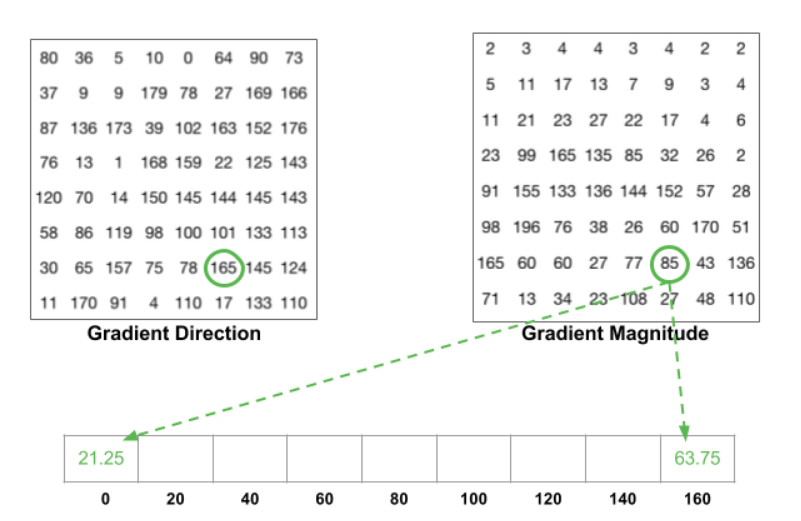
\includegraphics[height=60mm,width=120mm]{img/fig11.png}}
\caption{Mapping into 9-bin histogram array. Source: https://www.learnopencv.com}
\label{fig11}
\end{figure}

In the next step, we perform the block normalization. We take $16\times 16$ block, consisting of 4 cells. We calculate 9-bin histogram for each of the cell and concatenate all of them together which will produce a vector of dimension $36\times 1$. Now, to make the procedure more robust to lightning, we perform normalization on this $36\times 1$ vector by dividing each of its element with the L2 norm of the vector. For each $16\times 16$ block we calculate this vector and finally we concatenate them all together to get the HOG feature.


\section{Hybrid Deep Convolutional Neural Networks (HDNN)}
Deep convolutional neural networks is basically a CNN with a multi-layer perceptron (MLP) classifier. The CNN acts as a feature extractor and the MLP acts as a classifier. Here, CNN extracts feature of only one scale, i.e, it is not able to detect the ``large scale variance" \cite{b8} of objects. The objects show ``large scale variance" when they appear big in some images and small in some other images. CNN might not be able to detect this scale variance. 
\par Now, in this scenario HDNN \cite{b8} comes into the picture. Before describing the architecture of HDNN, let us introduce two definitions : 
\begin{itemize}
    \item \textbf{Source area: } Source area of a pixel in the output feature block is defined as the number of pixels from the input image that has been gone through each filter and resulted in that pixel in the output feature block. 
    \item \textbf{Feature scale: }It is the largest source area of a pixel in the output feature block from a CNN. 
\end{itemize}
\par Chen et.al \cite{b8} has used $7\times 7$ filters in convolution layer 1, $4\times 4$ filters in convolution layer 2 and also $4\times 4$ filters in convolution layer 3. Hence, the maximum source area of a pixel in the output feature block can be $28\times 28$. So, for each $28\times 28$ patch in the input image we will get one pixel in the output feature block. This shows that traditional CNN only extracts same scaled features. 
\par On the other hand, HDNN divides the last layer of convolution and pooling layers into $n_b$ number of blocks. Each block will be connected to the previous pooling layer. Each of the block has different filter size and max-pooling field size. Chen et. al \cite{b8} has divided the last layer into three blocks. First and second block has filter of size $4\times 4$. Thus the source area of the pixel of the feature block that will be resulted by these two blocks will be $28\times 28$. Whereas the third block has filter size $6\times 6$, which can indicate that the largest source area or feature scale of a pixel in the output feature block will be $36\times 36$. Hence, HDNN can extract features of different scales from the input images. The architecture of the HDNN is given in figure \ref{fig12}.

\begin{figure}[!htbp]
\centerline{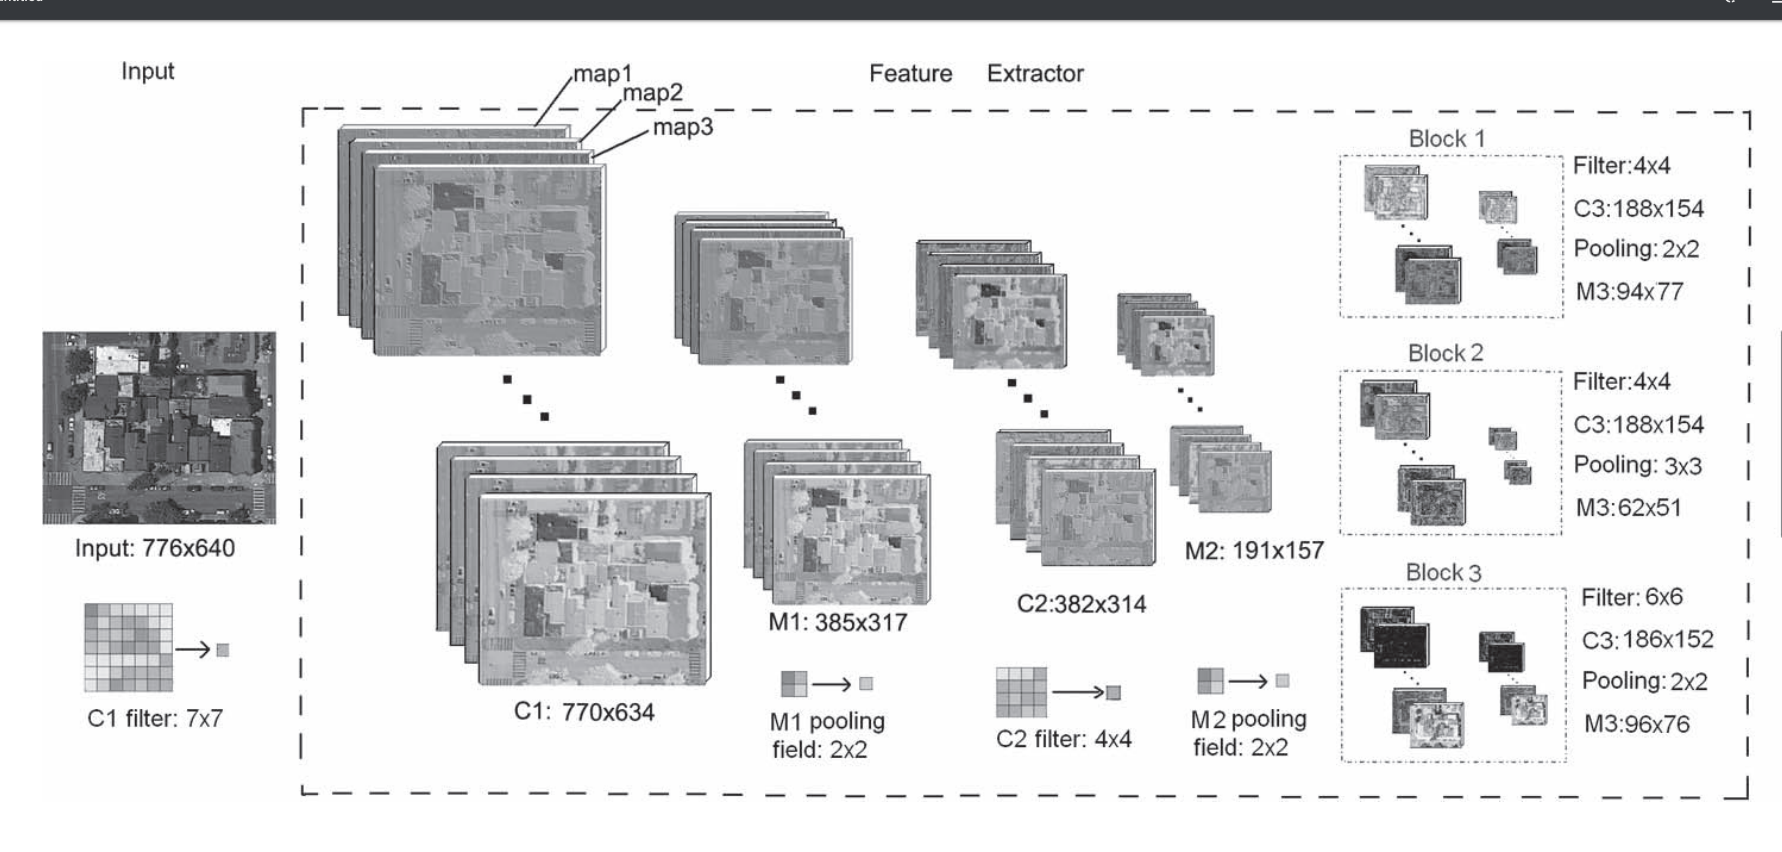
\includegraphics[height=80mm,width=140mm]{img/fig12.png}}
\caption{Architecture of HDNN. Source: \cite{b8}}
\label{fig12}
\end{figure}

\par These blocks having different filter sizes are responsible for producing the variable scaled feature vector of the object. 